
\chapter{Methods and Results}
\label{methods} % Always give a unique label
%use \chaptermark{}
% to alter or adjust the chapter heading in the running head

\section{Force Measurement}
\label{sec:sysArch}
Block diagram of the created system for 3-DOF force measurement is shown on figure \ref{fig:BlockDiag}. Forces that applied on the end of surgical tool are measured using strain gauges, which change their resistance with force. Using created printed circuit boards (PCBs), this resistance changes are measured and published within ROS. At the same time we measure current joint position of the tool, which is needed for the force calibration. On the PC position data and data from PCBs are used to find values of the force in X,Y,Z directions.

\begin{figure}[h]
	\begin{center}
		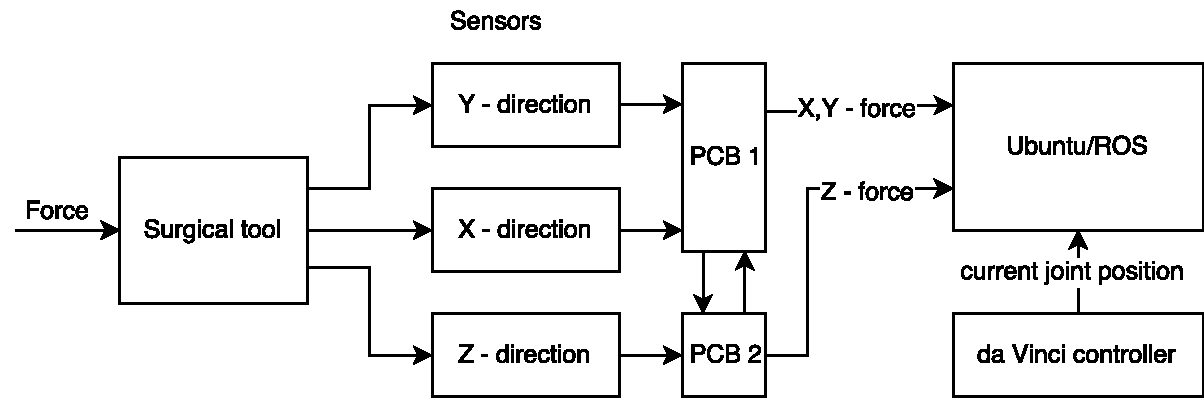
\includegraphics[width=140mm]{fig/methods/dbd2.pdf}
	\end{center}
	\vspace{-4mm}
	\caption[Block diagram]
	{Block diagram}
	\label{fig:BlockDiag}
	\vspace{-2mm}
\end{figure}

\section{Sensor Placement Optimization}
\label{sec:SimMod}
A finite element analysis was done in Solidworks to assess better placement of the strain gauges on the created device. In order to run finite element analysis material properties, such as elastic modulus, poisson`s ratio, and density are necessary to know. Sleeve material is aluminum 6061, that has elastic modulus 68.9 GPa, poisson`s ratio 0.33, and density 2700 kg/m\textsuperscript{3} \cite{aluminum_properties}. Since the shaft and cannula materials are unknown, in order to run finite element analysis their elasticity modulus and density were found experimentally.
	
	\subsection{Elastic Modulus Measurements}
	\label{sec:ElasMod}
	Elastic Modulus of the shaft and the cannula were found experimentally (Figure \ref{fig:ElasModSet}). One end of the observing sample (shaft/cannula) was fixed and the force was applied on the other end. We used weights 250g for the shaft and 555g for the cannula to apply forces. The deformation caused by forces was detected with dial indicator. Experiment was done 5 times, average displacement value was used to calculate elastic modulus. Results are shown in Table \ref{tab:elasMod}.
	
\begin{figure}[h]
	\begin{center}
		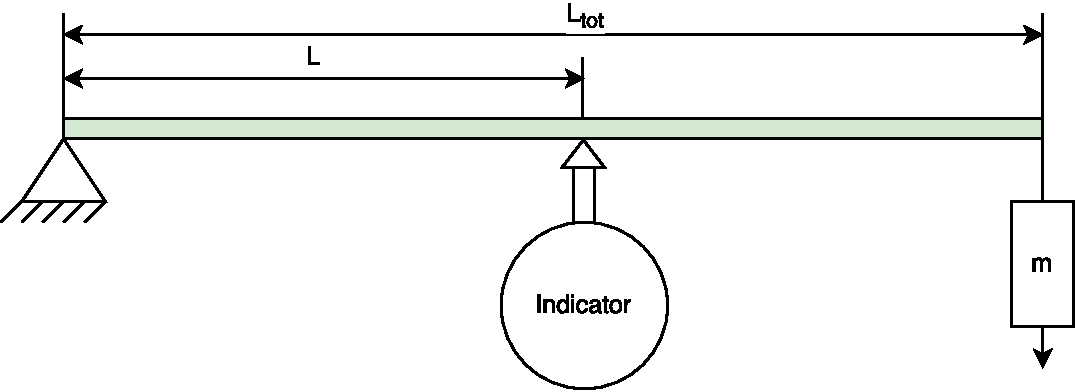
\includegraphics[width=120mm]{fig/methods/el_mod_set.pdf}
	\end{center}
	\vspace{-4mm}
	\caption[Setup to measure elasticity modulus]
	{Setup to measure elasticity modulus}
	\label{fig:ElasModSet}
	\vspace{-2mm}
\end{figure}

\begin{table}
\caption {Elasticity Modulus Measurement Data} \label{tab:elasMod} 
\begin{tabular}{ | c | c | c | c | c | c | c | c | } 
\hline
Component & $d_o$, mm & $d_i$, mm & $I$, mm\textsuperscript{4} & $m$, g & $F$, N & $L$, mm & $L_{tot}$, mm \\ 
\hline
Shaft & 8.4 & 6 & $1.808 \cdot 10^{-10}$ & 250 & 3.25 & 276.2 & 366.8\\ 
\hline
Cannula & 10.54 & 8.75 & $3.181 \cdot 10^{-10}$ & 555 & 6.011 & 95.5 & 105.55 \\ 
\hline
\end{tabular}

\begin{tabular}{ | c | c | c | } 
\hline
Component & $\delta \pm SD$, mm & $E \pm SD$, GPa \\ 
\hline
Shaft & $2.856 \pm 0.123$ & $44.31 \pm 1.86$ \\ 
\hline
Cannula & $0.086 \pm 0.004$ & $63.92 \pm 2.97$ \\ 
\hline
\end{tabular}
\end{table}

Elastic Modulus was found using following equation:

\begin{equation}
E = \frac{FL^3}{3 \delta I} 
\end{equation}

where $F$ - force, $L$ - length from the fixed point to indicator, $I$ - area moment of inertia, $\delta$ - displacement.

Area moment of Inertia: 
\begin{equation}
I = \frac{\pi (d_o^4 - d_i^4)}{64}
\end{equation}

where $d_o$ - cylinder outside diameter, $d_i$- cylinder inside diameter.

Force acting on indicator:
\begin{equation}
F = \frac{L_{tot}}{L}mg
\end{equation}

where $L_{tot}$ - total length of the object, $m$ - mass of the weight, $g$ - gravitational constant.

Experimentally found mean value of elastic modulus of the shaft is equal to 44.31 GPa with standard deviation (SD) 1.86 GPa, elastic modulus of the cannula is 63.92 GPa with SD 2.97 GPa, which is close to aluminum modulus of elasticity (68.9 GPa \cite{youngs_modulus}).

	\subsection{Density Measurements}
	\label{sec:DenMeas}
Density was found using following equation:

\begin{equation}
p=\frac{m}{V}
\end{equation}

where $m$ - mass, $V$ - volume.

Shaft material density is 3380 kg/m\textsuperscript{3}. From the elastic modulus of the cannula, we assumed that it is made of aluminum and consequently has density equal to 2700 kg/ m\textsuperscript{3}.

\subsection{Simulation Results}
\label{sec:FEAres}
From the Figure 2, it can be seen that the mounting location of the cannula seems to be under the greatest amount of strain. Additionally, the slight gap between the cannula and the DaVinci tool creates a large load point at the tip of the cannula as well as creating a slight moment of inaccuracy in readings at small loads. 

We suggest to place strain gauges at the mounting location of the cannula. Maximum strain is 0.46 mm, in case of 10N load with maximally opened shaft. From the literature, strain gauges length should be more than 5% of maximum strain, hence, minimum length of the strain gauge should be 9.2 mm. 

Gauge Factor (GF) for strain gauges usually is 2. According to the formula (4) strain gauge with resistance 120 Ω will give change in resistance 0.115 Ω, and 350 Ω - 0.338 Ω:
R=GFR,
where GF - gauge factor, R - resistance, - strain.

All material properties are listed in Table \ref{tab:matProp}.
\begin{table}
\caption {Material Properties} \label{tab:matProp} 
\begin{center}
\begin{tabular}{ | c | c | c | c | c | c | c | c | } 
\hline
Component & Elastic Modulus, GPa & Density, kg/ m\textsuperscript{3} \\ 
\hline
Shaft & 44.31 & 3380\\ 
\hline
Cannula & 63.92 & 2700 \\ 
\hline
Sleeve & 68.9 & 2700  \\ 
\hline
\end{tabular}
\end{center}
\end{table}

\section{Requirements for the Device}
	\label{sec:DevReq}
	From the literature review, following requiremetns for the device were developed:
	Biocompatibility
	
	Linearity
	
	Range of forces 
	Highest gripping force in Da Vinci tool was seen in the Hemo-lok[R] clip applier (39.92 [+ or -] 0.89 N).
	0.3 - 11 N. 
	Tensile strength and failure load of sutures for robotic surgery
	Others

\section{Mechanical Design}
\label{sec:mechDes}
At first we were rying to put sensors on the instrument shaft itself, on the cannula, on the sleeve to see where we get the most accurate results. 

	\subsection{Strain Gauge}
	\label{sec:SGReq}
	According to the manual for strain gauge selection provided by Vishay Micro-Measurements. The strain gauge should have following parameters:
	• Gauge length is 0.8 mm. Ideally gauge length should be 10 \% of the shaft radius;
	• Single grid;
	• Isoelastic (D alloy) that has higher gauge factor with E backing;
	• Encapsulated with pre attached leads;
	• Resistance – 120 Ohms;
	• Gauge factor - 2;
	• STC – number (self-temperature-compensation): DY – dynamic
	Since the diameter of the shaft is only 8.5 mm, one of the most important parameters, in this
	case, is the size of the strain gauge. Another important parameter is gauge‘s resistance, sensitivity
	of the strain gauge drastically depends on this parameter. Strain gauges with different resistivity
	were used (350 and 120 Ohms and sizes of 6 x 2.5 mm).

	\subsection{Installation of Strain Gauges}
	\label{sec:instSG}

	The shaft was assumed to be made of Tecamax, but for gauge installation purposes materials for plastic was chosen as it is comparable in preparation. \cite{StrGugeInst}.

	First the working surface (glass) and tweezers were cleaned with Neutralizer 5. After that shaft surface preparation was started, using solvent degreaser GC-6 Isopropyl Alcohol. A gauge layout was then applied with a 4H drafting pencil. The surface was then conditioned with Conditioner A and the extra liquid was wiped with gauze. Finally, the surface was then neutralized with M-Prep Neutralizer 5A. \cite{StrGugeInst}

	The strain gauges were first placed on the glass and then transported using mylar tape onto the instrument surface. A thin layer of catalyst was applied on the strain gauge and given one minute to dry. Then adhesive M-BOND 200 was applied on the shaft, pressure was applied on the tape for one minute, then two more minutes to let it dry before the tape was removed. Then leads soldering was done by application of pats, and soldering them with thin wires. \cite{youtube}

	The methodology of the strain gauge application more specifically described in \cite{StrGugeInst}.

	In compliance with the literature \cite{StrGugeInst} for application of the strain gauge on metals, the same materials and technique can be used. Therefore, the same method to apply strain gauges on the cannula was used.

	On the shaft
	On the cannula
	On the aluminum sleeve
	On the nylon sleeve

\subsection{Sensors on the tool and the cannula}
\label{sec:senOnToolCan}


\subsection{X-Y direction}
\label{sec:xyDir}
Do not use 3D printed sleeves - causes non-linearity issue
Use 350 Ohm strain-gauges and full-bridge circuit.
	
\subsection{Z-direction}
\label{sec:zDir}
\begin{figure}
	\begin{center}
		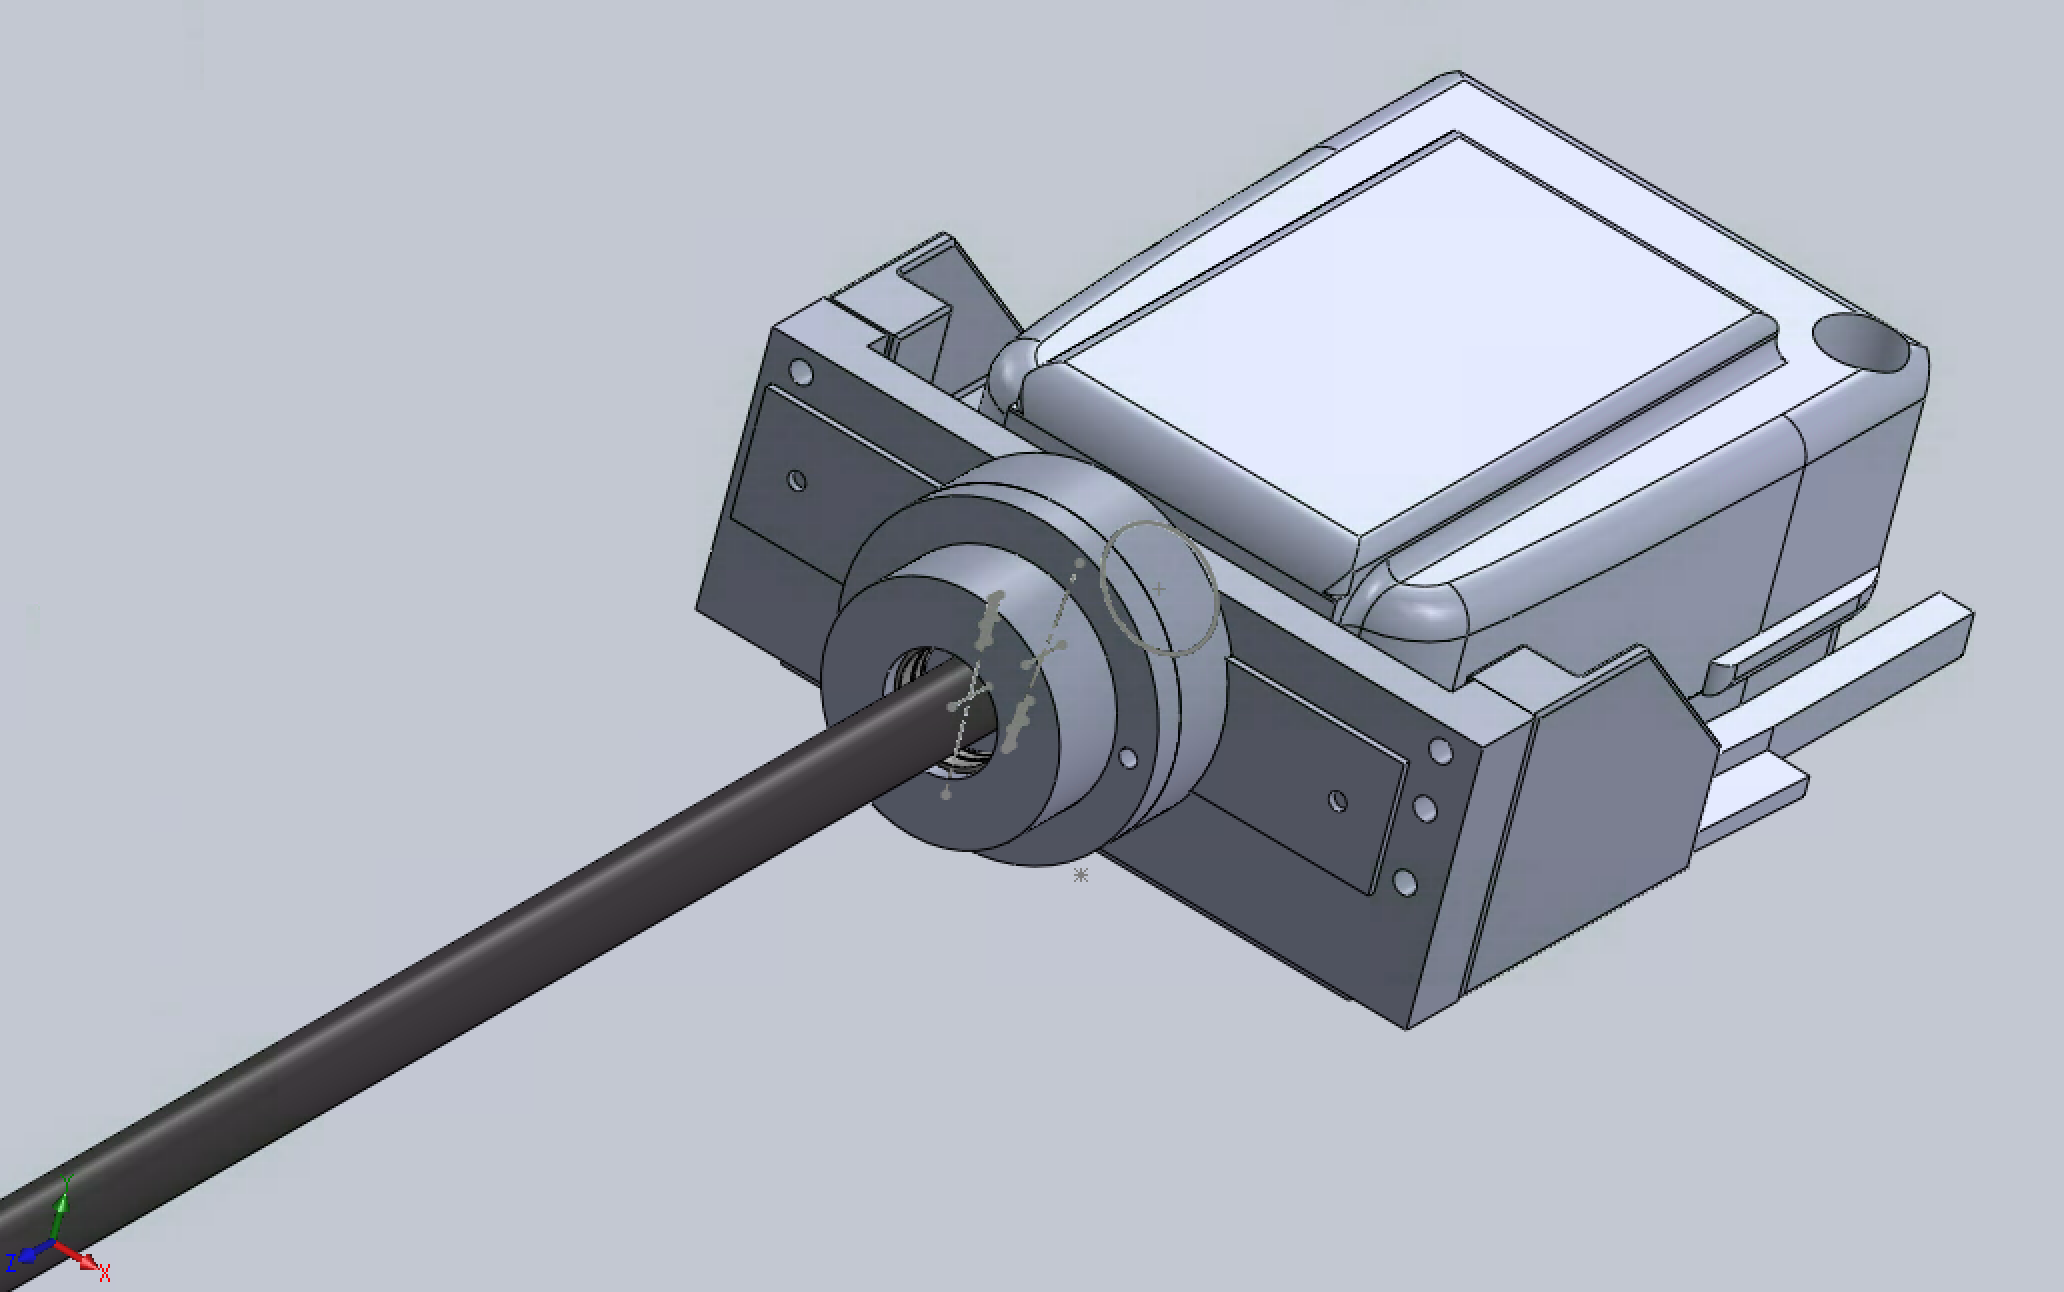
\includegraphics[width=120mm]{fig/methods/z_dir.png}
	\end{center}
	\vspace{-4mm}
	\caption[Z-direction force feedback sensor]
	{Z-direction force feedback sensor}
	\label{fig:Z-direction}
	\vspace{-2mm}
\end{figure}

\begin{figure}
	\begin{center}
		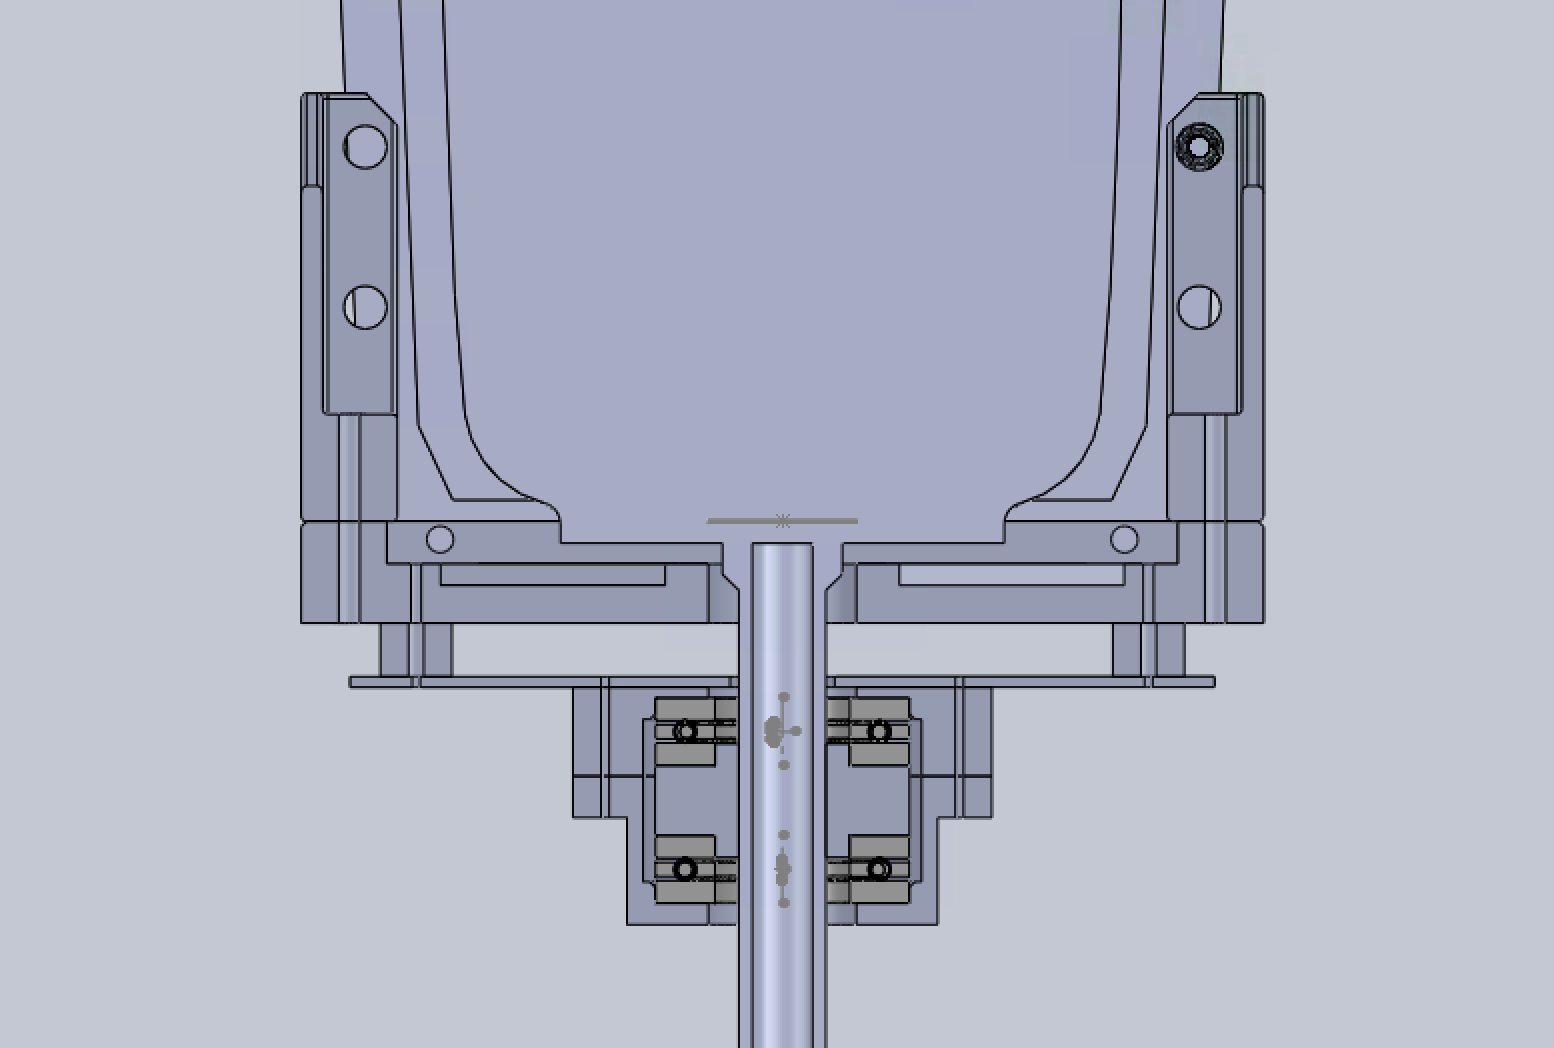
\includegraphics[width=120mm]{fig/methods/z_dir_sec.png}
	\end{center}
	\vspace{-4mm}
	\caption[Z-direction force feedback sensor - section vew]
	{Z-direction force feedback sensor - section vew}
	\label{fig:Z-direction_sec}
	\vspace{-2mm}
\end{figure}


\section{Electrical and Software Design}
\label{sec:elecDes}

Using Altium Designer 15.1 PCB was developed and manufactured elsewhere. 

Write about how to calibrate the PCB itself and how it works.

	\subsection{Circuit design}
	\label{sec:cirDes}
	Write about how circuit works.

	\subsection{Noise Analysis}
	\label{sec:NoiseExp}
	Noise analysis was performed using oscilloscope ... Make FFT analysis

		\begin{figure}[h]
			\begin{center}
			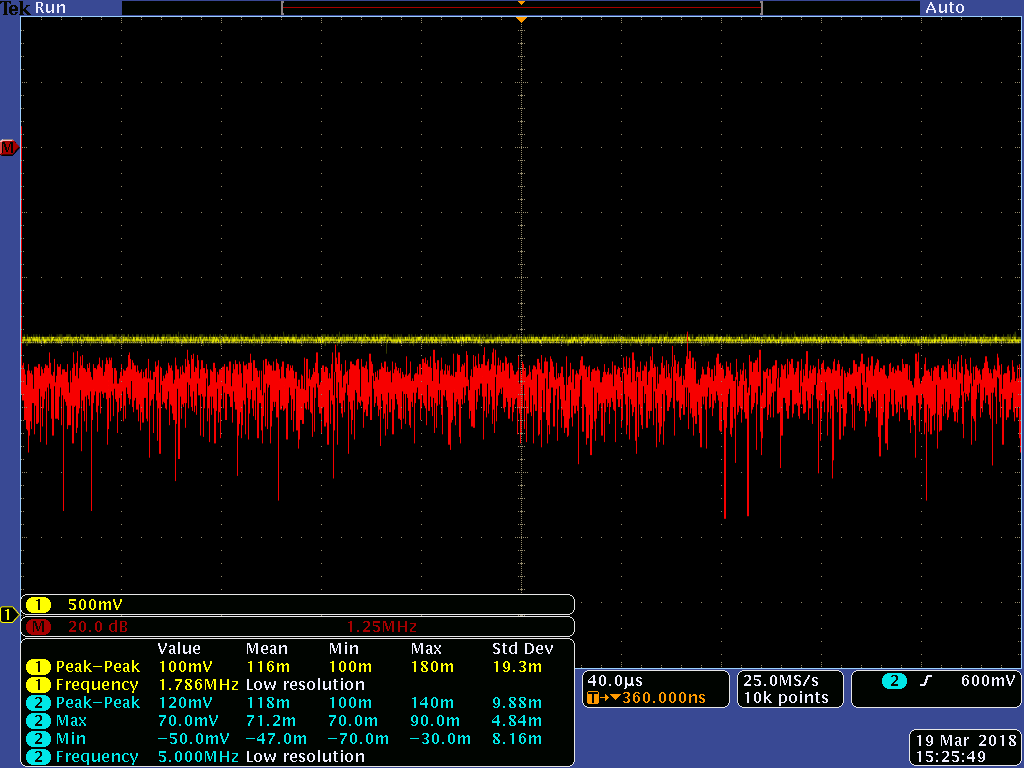
\includegraphics[width=120mm]{fig/results/40us_1stADC.png}
			\end{center}
			\vspace{-4mm}
		\caption[Noise analysis of the output signal]
		{Noise analysis of the output signal}
		\label{fig:OutputSignal}
		\vspace{-2mm}
		\end{figure}

	\subsection{Microcontroller Software}
	\label{sec:MicrSoft}
	We use arduino for ..
	Filtering was implemented on microcontroller by finding average of recent 5 readings 
	Filtering - ideally small time delay. Total teleoperation cycle delay - less than 100ms (visually noticeable delay). Kalman filter? Use same parameters for both signals to get identical time delay.
	good article about changing baud rate.

	\subsection{ROS Architecture}
	\label{sec:p2}
	
\section{Calibration}
\label{section:Calibration}
First we used set of weights applied in two directions, but since the system was too sensitive for direction of force, we had to change our approach of determining the force direction. It was decided to use optical tracking system for that purpose.

	\subsection{Calibration Setup}
	\label{sec:CalSetup}
	Tell how calibration with optical tracking system is working

	\subsection{Calibration of the Load Cell}
	\label{sec:CalLoadCell}
	Was pefrormed using following setup cite figure ..
	Calibration equation we got ..

	\subsection{Calibration Results}
	Find mean square root error

		\begin{figure}
			\centering
			\begin{subfigure}
				\centering
				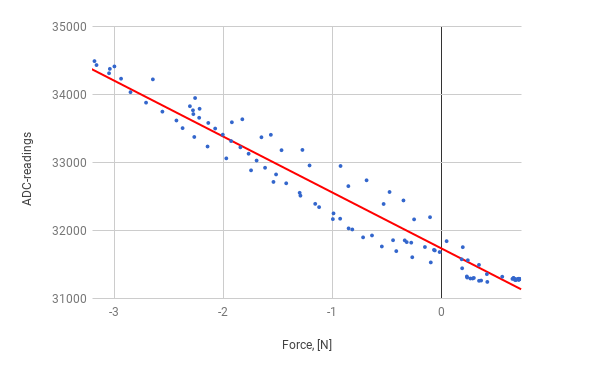
\includegraphics[width=120mm]{fig/results/x-dir.png}
				\caption{X-component}
				\label{fig:Xdirection}
			\end{subfigure}
			\begin{subfigure}
				\centering
				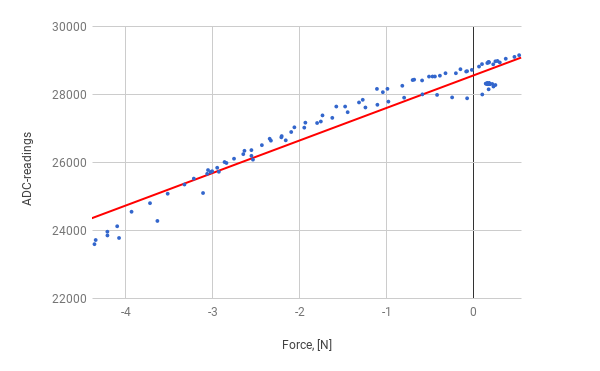
\includegraphics[width=120mm]{fig/results/y-dir.png}
				\caption{Y-component}
				\label{fig:Ydirection}
			\end{subfigure}
			\caption{Calibration results}
			\label{fig:Calibration}
		\end{figure}

\section{Experiments}
\label{sec:Experims}

	\subsection{Distance from the cannula to the tip dependence from readings}
	\label{sec:DisExp}
	Distance from the cannula to the tip - measure - 3 ¼ inch. Maximum distance is 9 inches.


	\subsection{Temeperature Dependence}
	\label{sec:TempExp}
	Try in 36.6 Celsius and room temperature
	Effect of the surrounding temperature on the device was ..

	Do all experiments at least three times and calculate all statistic things you can (SD)

	\subsection{Hysteresis}
	\label{sec:HystExp}
	Hysteresis was checked .. 
	We written separate program to check hysteresis
	
\subsection{Static Characteristics}
\label{sec:StatCharac}
Precision represents capacity of a sensing system to give the same reading when repetitively measuring the same measurand under the same conditions. The precision is a statistical parameter and can be assessed by the standard deviation (or variance) of a set of readings of the system for similar inputs.

One of the measurements of signal quality is signal-to-noise ratio (SNR). A higher value of SNR means the clear acquisitions with low signal distortions and artifacts caused by unwanted noise. It is defined as:

\begin{equation}
\frac{S}{N}=\frac{Mean value of signal}{Standard deviation of noise}
\end{equation}

For X-direction SNR is $3232 \pm 78$, for Y-direction SNR is $2857 \pm 150$, which is much bigger than 1. It means that system has very low noise.

Error is the difference between the actual value of the measurand and the value produced by the sensing system. Error can be caused by a variety of internal and external sources and is closely related to accuracy. Accuracy can be related to absolute or relative error as:

\begin{equation}
Absolute error = \frac{Output}{ True value}
\end{equation}

\begin{figure}
	\begin{center}
		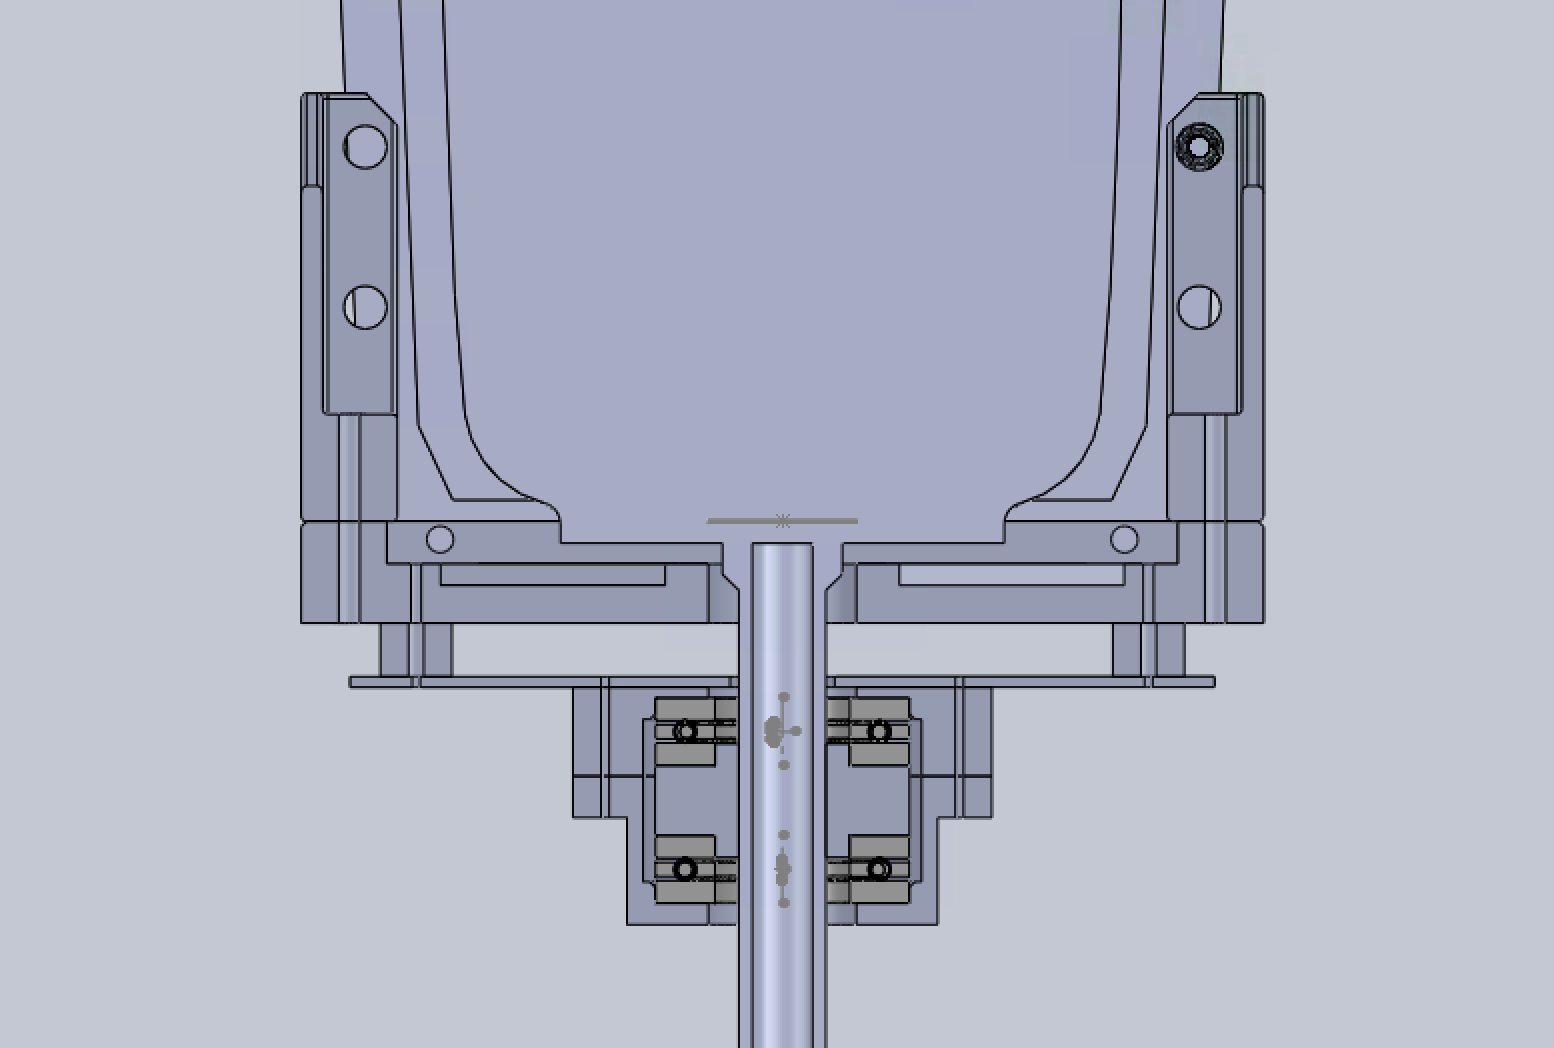
\includegraphics[width=120mm]{fig/methods/z_dir_sec.png}
	\end{center}
	\vspace{-4mm}
	\caption[Z-direction force feedback sensor - section vew]
	{Z-direction force feedback sensor - section vew}
	\label{fig:Z-direction_sec}
	\vspace{-2mm}
\end{figure}

From figure we can assume that fluctuations in the output signal are due to systematic errors. 

Drift is observed when a gradual change in the sensing system’s output is seen, while the measurand actually remains constant. Drift is the undesired change that is unrelated to the measurand. It is considered a systematic error, which can be attributed to interfering parameters such as mechanical instability and temperature instability, contamination, and the sensor’s materials degradation. 

Resolution (or discrimination) is the minimal change of the measurand that can produce a detectable increment in the output signal. Resolution is strongly limited by any noise in the signal.

In a sensing system, minimum detectable signal (MDS) is the minimum signal increment that can be observed, when all interfering factors are taken into account. When the increment is assessed from zero, the value is generally referred to as threshold or detection limit. If the interferences are large relative to the input, it will be difficult to extract a clear signal and a small MDS cannot be obtained.

Sensitivity is the ratio of the incremental change in the sensor’s output (Dy) to the incremental change of the measurand in input (Dx). The slope of the calibration curve, y f(x), can be used for the calculation of sensitivity.

The closeness of the calibration curve to a specified straight line shows the linearity of a sensor. Its degree of resemblance to a straight line describes how linear a system is.

Hysteresis is the difference between output readings for the same measurand, depending on the trajectory followed by the sensor.

The maximum and minimum values of the measurand that can be measured with a sensing system are called the measurement range, which is also called the dynamic range or span. This range results in a meaningful and accurate output for the sensing system. \cite{kalantar-zadeh_sensors_2013}




